% !TEX TS-program = lualatex
% !TEX encoding = UTF-8 Unicode

\documentclass[12pt, letterpaper]{article}

%%BIBLIOGRAPHY- This uses biber/biblatex to generate bibliographies according to the
%%Unified Style Sheet for Linguistics
\usepackage[main=american, german]{babel}% Recommended
\usepackage{csquotes}% Recommended
\usepackage[backend=biber,
        style=unified,
        maxcitenames=3,
        maxbibnames=99,
        natbib,
        url=false,
        doi=false]{biblatex}
\addbibresource{Dissertation.bib}
\setcounter{biburlnumpenalty}{100}  % allow URL breaks at numbers
% \setcounter{biburlucpenalty}{100}   % allow URL breaks at uppercase letters
% \setcounter{biburllcpenalty}{100}   % allow URL breaks at lowercase letters
\AtBeginBibliography{\footnotesize}

%%TYPOLOGY
\usepackage[svgnames]{xcolor} % Specify colors by their 'svgnames', for a full list of all colors available see here: http://www.latextemplates.com/svgnames-colors
%\usepackage[compact]{titlesec}
%\titleformat{\section}[runin]{\normalfont\bfseries}{\thesection.}{.5em}{}[.]
%\titleformat{\subsection}[runin]{\normalfont\scshape}{\thesubsection}{.5em}{}[.]
\usepackage[hmargin=2.5cm,vmargin=2.5cm]{geometry}  %Margins          
\usepackage{graphicx}	%Inserting graphics, pictures, images 		
\usepackage{stackengine} %Package to allow text above or below other text, Also helpful for HG weights 
\usepackage{fontspec} %Selection of fonts must be ran in XeLaTeX or LuaLateX
\usepackage{amssymb} %Math symbols
\usepackage{amsmath} % Mathematical enhancements for LaTeX
\usepackage{setspace} %Linespacing
\usepackage{multicol} %Multicolumn text
\usepackage{enumitem} %Allows for continuous numbering of lists over examples, etc.
\usepackage{multirow} %Useful for combining cells in tablesbrew 
\usepackage{hanging}
\usepackage{fancyhdr} %Allows for the 
% \pagestyle{fancy}
\fancyhead[L]{\textit{TITLE}} 
\fancyhead[R]{\textit{\today}} 
\fancyfoot[L,R]{} 
\fancyfoot[C]{\thepage} 
\renewcommand{\headrulewidth}{0.4pt}
\setlength{\headheight}{14.5pt} % ...at least 14.49998pt
% \usepackage{fourier} % This allows for the use of certain wingdings like bombs, frowns, etc.
% \usepackage{fourier-orns} %More useful symbols like bombs and jolly-roger, mostly for OT
\usepackage[colorlinks,allcolors={black},urlcolor={blue}]{hyperref} %allows for hyperlinks and pdf bookmarks
% \usepackage{url} %allows for urls
% \def\UrlBreaks{\do\/\do-} %allows for urls to be broken up
\usepackage[normalem]{ulem} %strike out text. Handy for syntax
\usepackage{tcolorbox}
\usepackage{todonotes} % Creates todo marginalia

%%FONTS
\newfontfamily{\ipa}{Doulos SIL}
\setmainfont{Libertinus Serif}
\setsansfont{Libertinus Sans}
\setmonofont[Scale=MatchLowercase]{Libertinus Mono}

%%PACKAGES FOR LINGUISTICS
%\usepackage{OTtablx} %Generating tableaux with using TIPA
% \usepackage[noipa]{OTtablx} % Use this one generating tableaux without using TIPA
%\usepackage[notipa]{ot-tableau} % Another tableau drawing packing use for posters.
\usepackage{linguex} % Linguistic examples
% \usepackage{langsci-linguex} % Linguistic examples
% \usepackage{langsci-gb4e} % Language Science Press' modification of gb4e
% \usepackage{langsci-avm} % Language Science Press' AVM package
\usepackage{tikz} % Drawing Hasse diagrams
% \usepackage{pst-asr} % Drawing autosegmental features
\usepackage{pstricks} % required for pst-asr, OTtablx, pst-jtree.
% \usepackage{pst-jtree} 	% Syntax tree draawing software
% \usepackage{tikz-qtree}	% Another syntax tree drawing software. Uses bracket notation.
\usepackage[linguistics]{forest}	% Another syntax tree drawing software. Uses bracket notation.
% \usepackage{ling-macros} % Various linguistic macros. Does not work with linguex.
% \usepackage{covington} % Another linguistic examples package.
\usepackage{leipzig} %	Offers support for Leipzig Glossing Rules

%%LEIPZIG GLOSSING FOR ZAPOTEC
\newleipzig{el}{el}{elder} % Elder pronouns
\newleipzig{hu}{hu}{human} % Human pronouns
\newleipzig{an}{an}{animate} % Animate pronouns
\newleipzig{in}{in}{inanimate} % Inanimate pronouns
\newleipzig{pot}{pot}{potential} % Potential Aspect
\newleipzig{cont}{cont}{continuative} % Continuative Aspect
\newleipzig{stat}{stat}{stative} % Stative Aspect
\newleipzig{and}{and}{andative} % Andative Aspect
\newleipzig{ven}{ven}{venative} % Venative Aspect
% \newleipzig{res}{res}{restitutive} % Restitutive Aspect
\newleipzig{rep}{rep}{repetitive} % Repetitive Aspect

%%TITLE INFORMATION
\title{SSLA 4 Abstract}
% \author{Mykel Loren Brinkerhoff}
\date{\today}

%%MACROS
\newcommand{\sub}[1]{\textsubscript{#1}}
\newcommand{\supr}[1]{\textsuperscript{#1}}
\providecommand{\lsptoprule}{\midrule\toprule}
\providecommand{\lspbottomrule}{\bottomrule\midrule}
\newcommand{\fittable}[1]{\resizebox{\textwidth}{!}{#1}}

\makeatletter
\renewcommand{\paragraph}{%
  \@startsection{paragraph}{4}%
  {\z@}{0ex \@plus 1ex \@minus .2ex}{-1em}%
  {\normalfont\normalsize\bfseries\itshape}%
}
\makeatother
\parindent=10pt


\begin{document}

%%If using linguex, need the following commands to get correct LSA style spacing
%% these have to be after  \begin{document}
    % \setlength{\Extopsep}{6pt}
    % \setlength{\Exlabelsep}{9pt}		%effect of 0.4in indent from left text edge
%%

%% Line spacing setting. Comment out the line spacing you do not need. Comment out all if you want single spacing.
%	\doublespacing
%	\onehalfspacing

\begin{center}
    \textbf{Measuring voice quality in Zapotec}
\end{center}

\paragraph{Introduction:} Voice quality (VQ) refers to the manner in which phonation occurs. It is widely employed in the world's languages for both paralinguistic and phonological contrasts (see \cite{garellekPhoneticsVoice2019} for an overview). It has long been established that VQ has acoustic correlates in the signal \citep{fischer-jorgensenPhoneticAnalysisBreathy1968}. The most commonly used of these acoustic measures being H1-H2.

Recent research by \citet{chaiH1H2Acoustic2022} shows that H1-H2 is less robust and is prone to error propogation. They propose using a Residual H1*, which factors out the root mean squared energy from H1*. They show that this measure is more robust and better captures the VQ distinctions in !Xõó and Mandarin Chinese than H1*-H2*.

Building on this research into residual H1*, \citet{brinkerhoffResidualH1Measure2024} show that residual H1* better captures the VQ distinctions in Santiago Laxopa Zapotec. The present study validates those findinigs using generalized additive mixed models, which better account for dynamic data, such as changes in harmonic amplitude, than linear regression models \citep{hastieGeneralizedAdditiveModels1986,wielingAnalyzingDynamicPhonetic2018,soskuthyEvaluatingGeneralisedAdditive2021}. 

\paragraph{Santiago Laxopa Zapotec (SLZ):} SLZ is an indigenous language from Santiago Laxopa, Ixtlán, Oaxaca, Mexico and spoken by $\sim$1000 speakers.  This variety is unique for being a Northern Core Zapotec that has developed breathy voice (B; 1b) in addition to the two types of laryngealization that characterize the rest of the Zapotecan languages, namely checked (C; 1c) and rearticulated (R; 1d) (see \cite{ariza-garciaPhonationTypesTones2018} for a detailed typology of VQ in Zapotec languages). This contrast can be seen in the near minimal quadruple in (1a-d).
\ex.
  \begin{multicols}{2}
    \a. \textit{ya} [{\ipa ʝa˦} ] ‘temazcal’
    \b. \textit{yah} [{\ipa ʝa̤˨}] ‘iron’
    \b. \textit{cha’} [{\ipa tʃaˀ˨}] ‘pot’ 
    \b. \textit{ya’a} [{\ipa ʝaˀa˨}] ‘market’
    \z.
  \end{multicols}
\z.

SLZ additionally has three tones and two contours independent of the VQ contrast.This results in VQ and tone being orthogonal to each, which complicates acoustical analyses into SLZ.  
\paragraph{Methodology:} A word list elicitation was collected from 10 native SLZ speakers (five female) in Santiago Laxopa, Oaxaca. This word list contained 76 words across the four VQ contrasts. Each word was said in isolation and a carrier sentence three times. The vowels from the carrier sentences were segmented following \citet{garellekAcousticDiscriminabilityComplex2020}, and processed using VoiceSauce \citep{shueVOICESAUCEProgramVoice2009}. Several measures were assessed in this study: corrected H1*-H2*, Residual H1* as discussed in \citet{chaiH1H2Acoustic2022}, and corrected H1*-A3, following previous work on this variety \citep{adlerAcousticsPhonationTypes2016}.  Three generalized additive mixed models (GAMMs; \cite{hastieGeneralizedAdditiveModels1986}) were fitted, one each for H1*-H2*, H1*-A3, and residual H1*.

\paragraph{Results:} Figure~1 shows H1*-H2* and that each of the non-modal VQs have lower values than M and they overlap in each of the three vowel positions. Figure~2 shows that the only contrasts reliably captured by H1*-A3 are B, C, and M; R and M are nearly identical throughout the vowel. Figure~3 shows that residual H1* reliably separates B, C, and R from M, and also captures the positional distinction between R and C. The three GAMMs support the visualizations.

\paragraph{Conclusion:} The results of this study on Santiago Laxopa Zapotec confirms the findings of \citet{brinkerhoffResidualH1Measure2024} and shows that residual H1* is a reliable measures of VQ and should be considered when assessing phonation type in languages with complex phonation systems like Zapotec.


%------------------------------------
%BIBLIOGRAPHY
%------------------------------------
\newpage
% \begin{figure}[htbp]
%   \centering
%   \begin{minipage}{.5\textwidth}
%     \centering
%     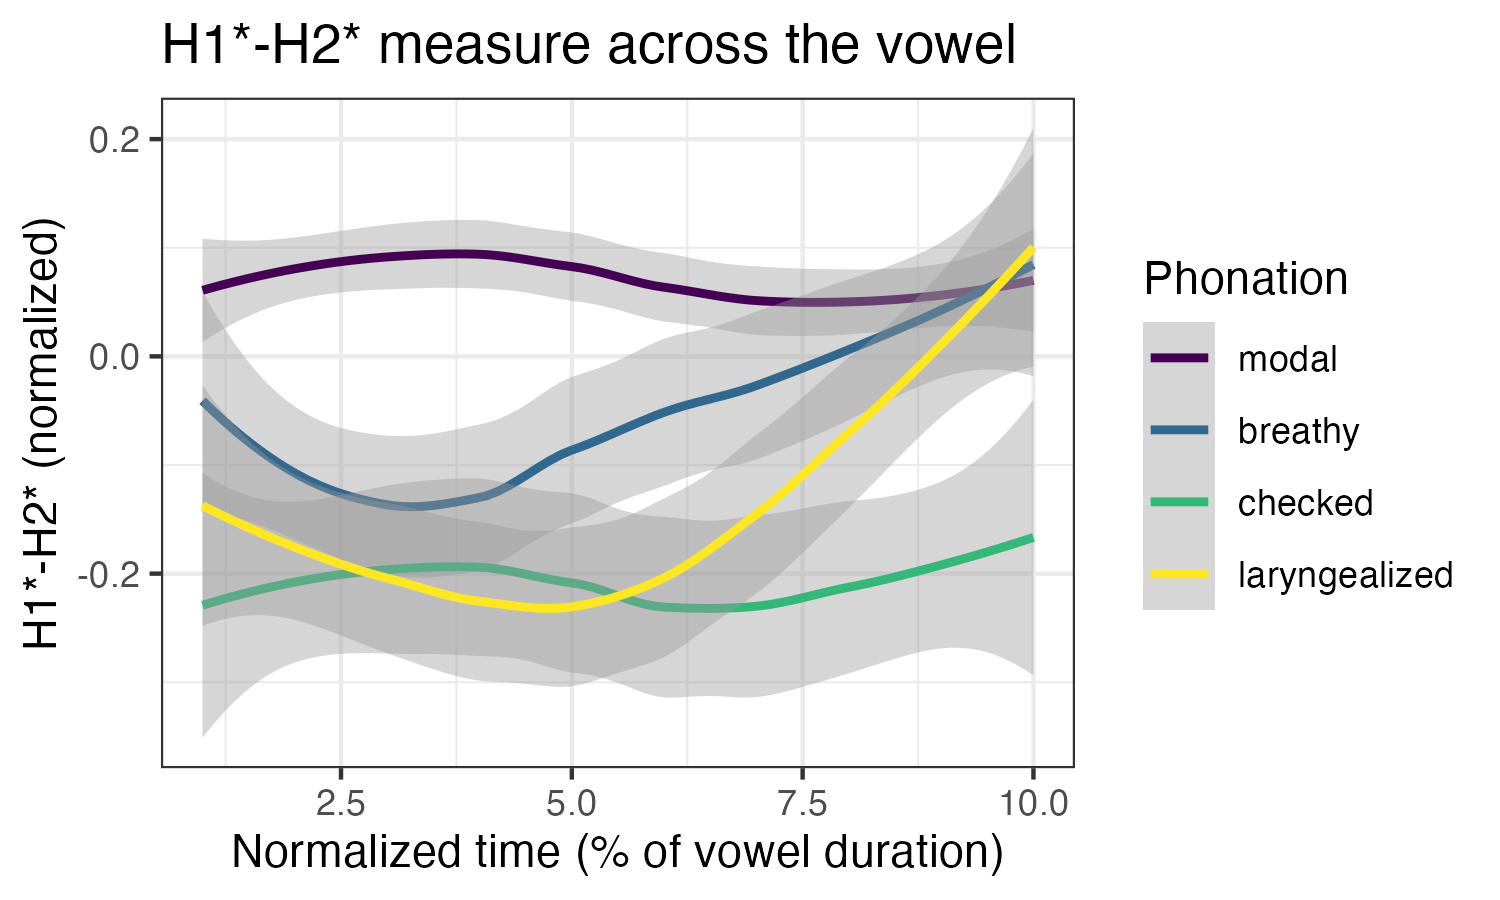
\includegraphics[width=.33\linewidth]{Images/h1h2_clean_line.png}
%     \caption{Genelec 8010 AP}
%   \label{fig:Genelec 8010}
%   \end{minipage}%
%   \begin{minipage}{.5\textwidth}
%     \centering
%     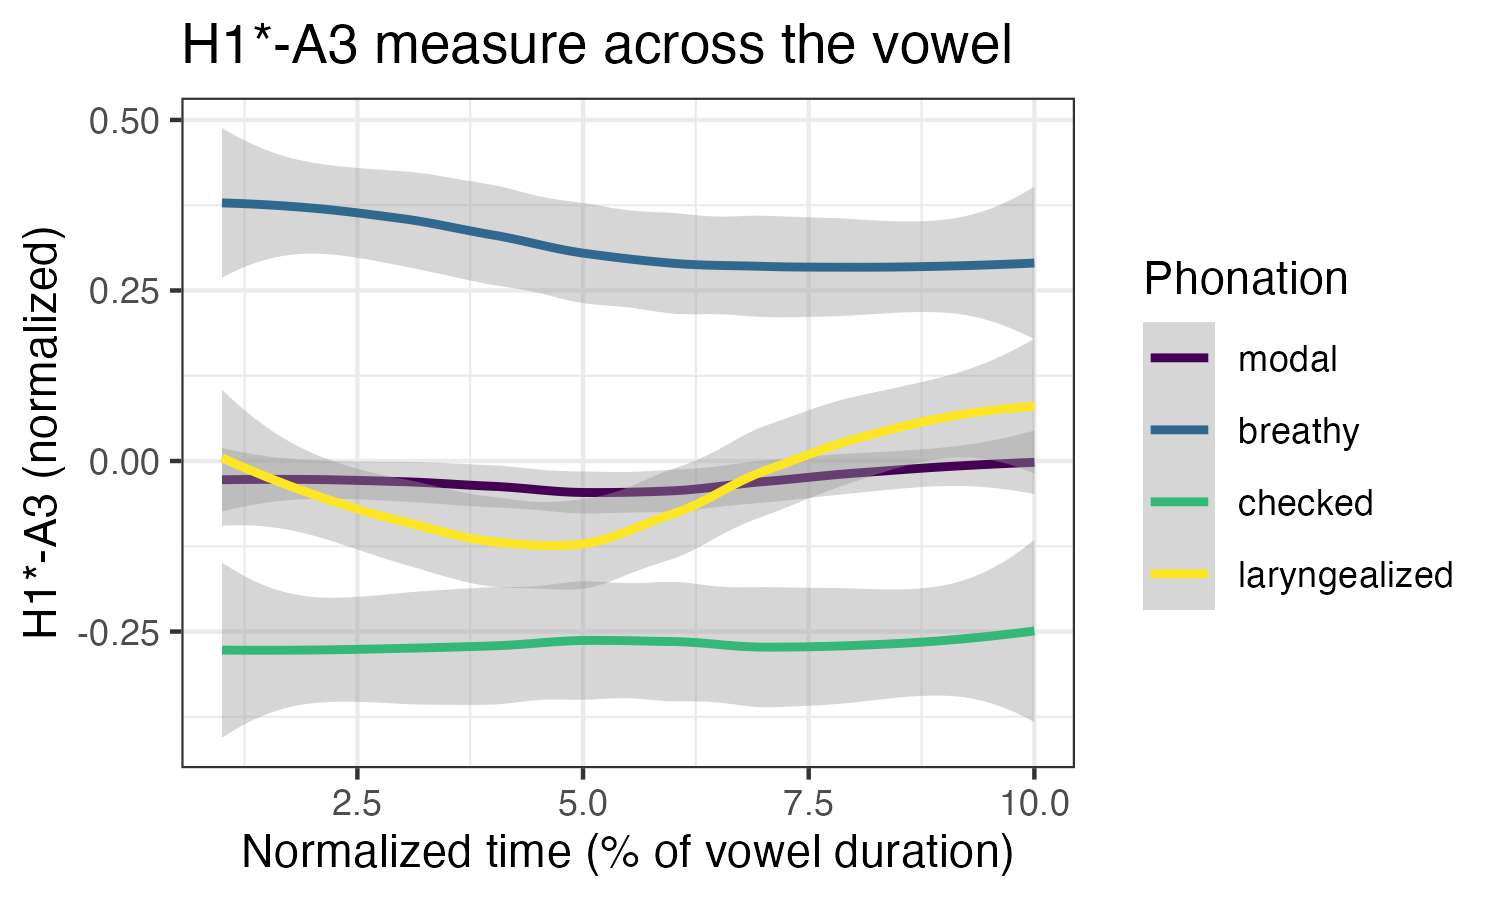
\includegraphics[width=.33\linewidth]{Images/h1a3_clean_line.png}
%     \caption{Genelec 8020 CPM}
%     \label{fig:Genelec 8020}
%   \end{minipage}%
%   \begin{minipage}{.5\textwidth}
%     \centering
%     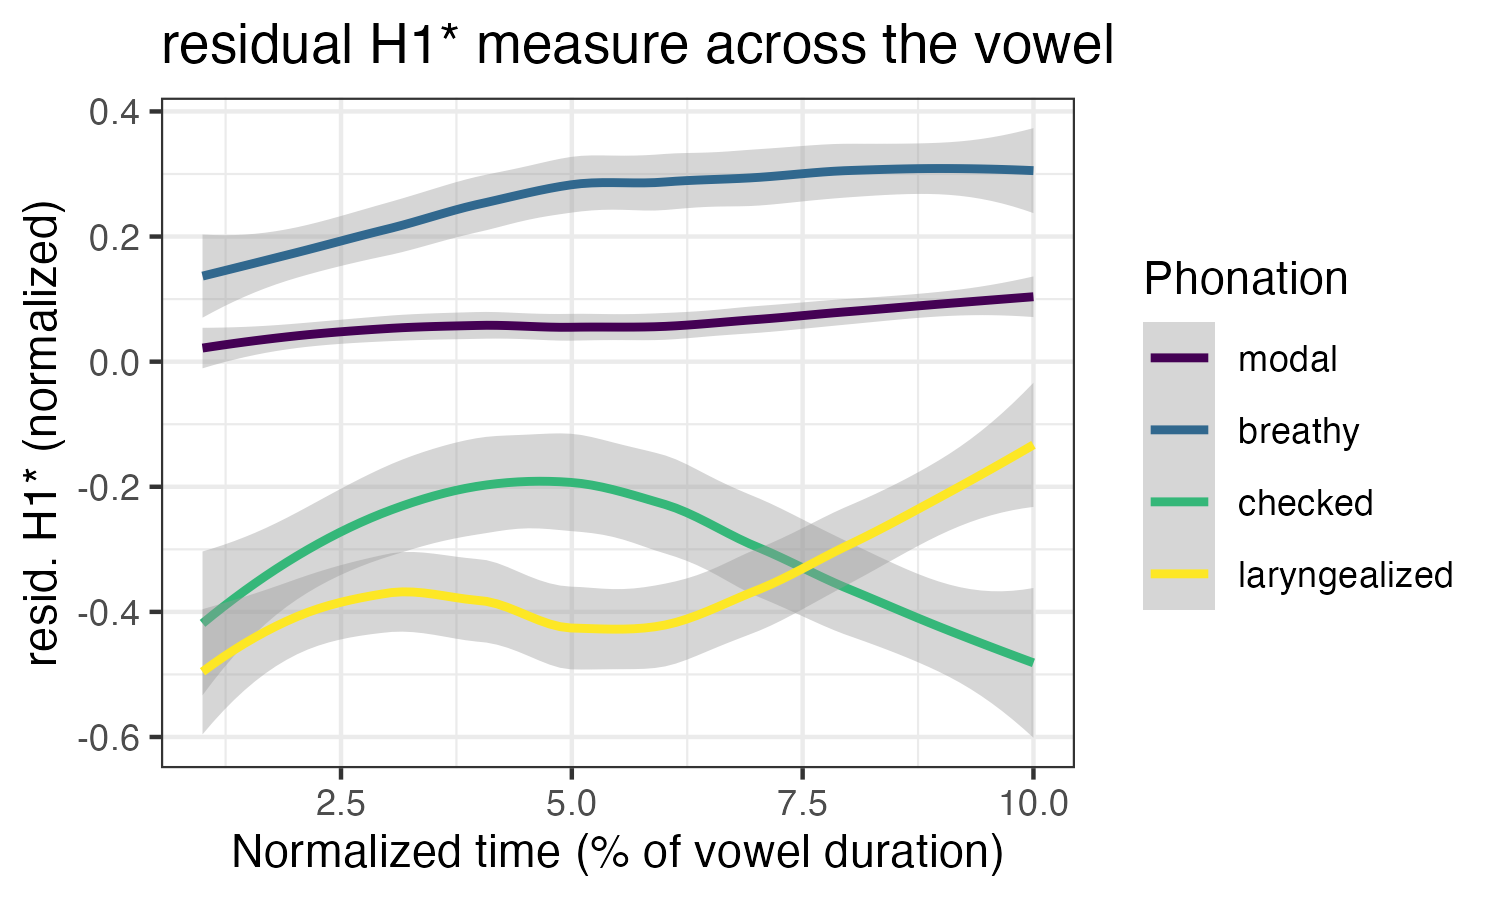
\includegraphics[width=.33\linewidth]{Images/h1_clean_line.png}
%     \caption{Genelec 8020 CPM}
%     \label{fig:Genelec 8020}
%   \end{minipage}%
% \end{figure}

\begin{figure}[htp]% [H] is so declass\'e!
  \centering
  \begin{minipage}{0.45\textwidth}
  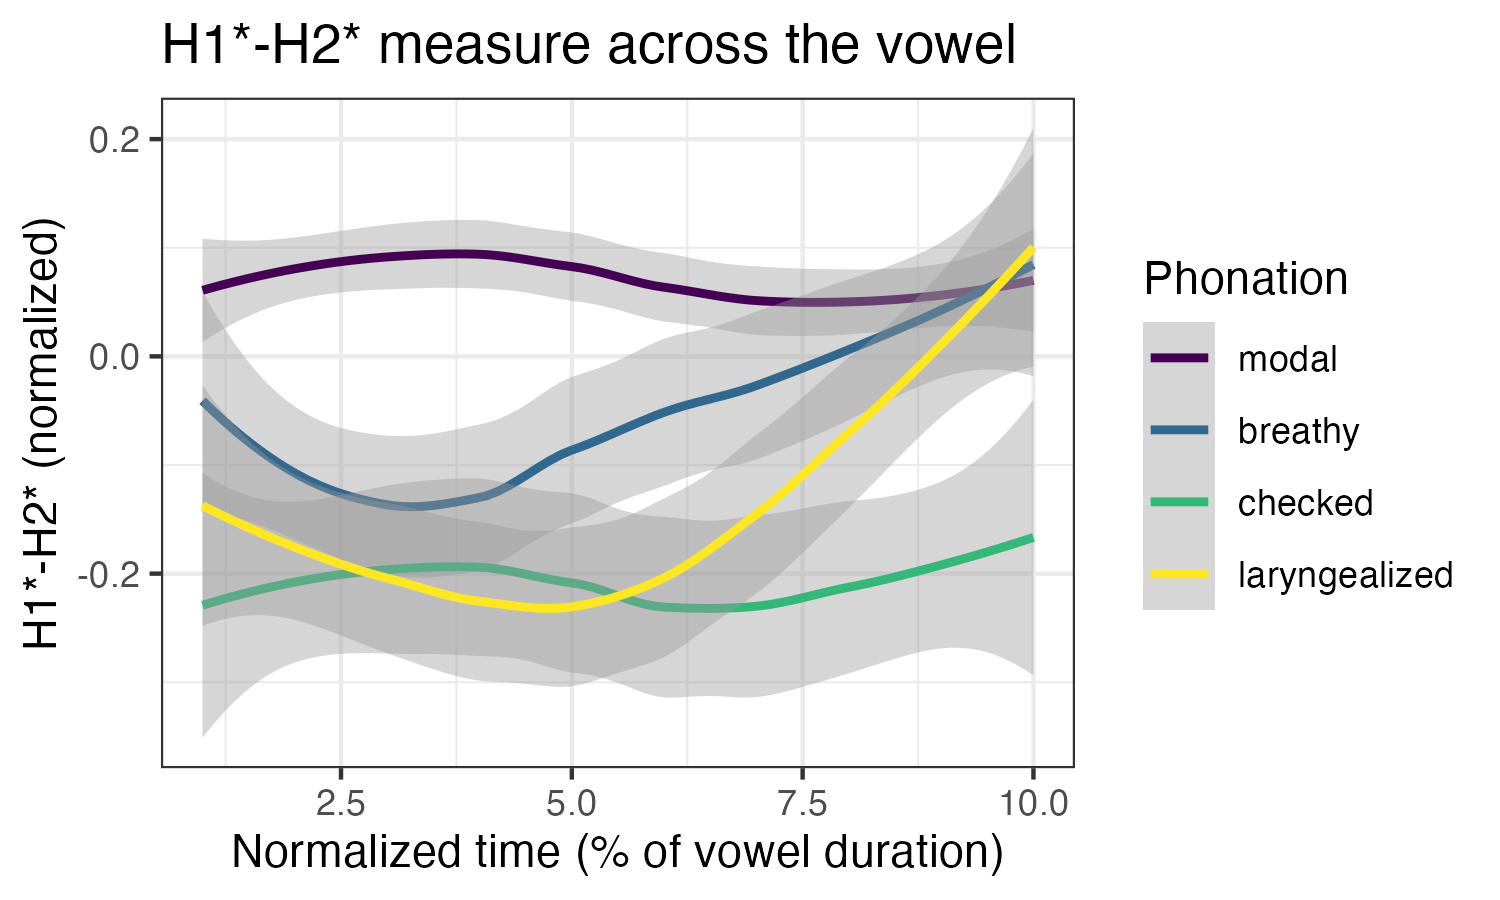
\includegraphics[width=\textwidth]{Images/h1h2_clean_line.png}
  \caption{Smooths for H1*-H2* by phonation contrast}
  \end{minipage}\hfill
  \begin{minipage}{0.45\textwidth}
  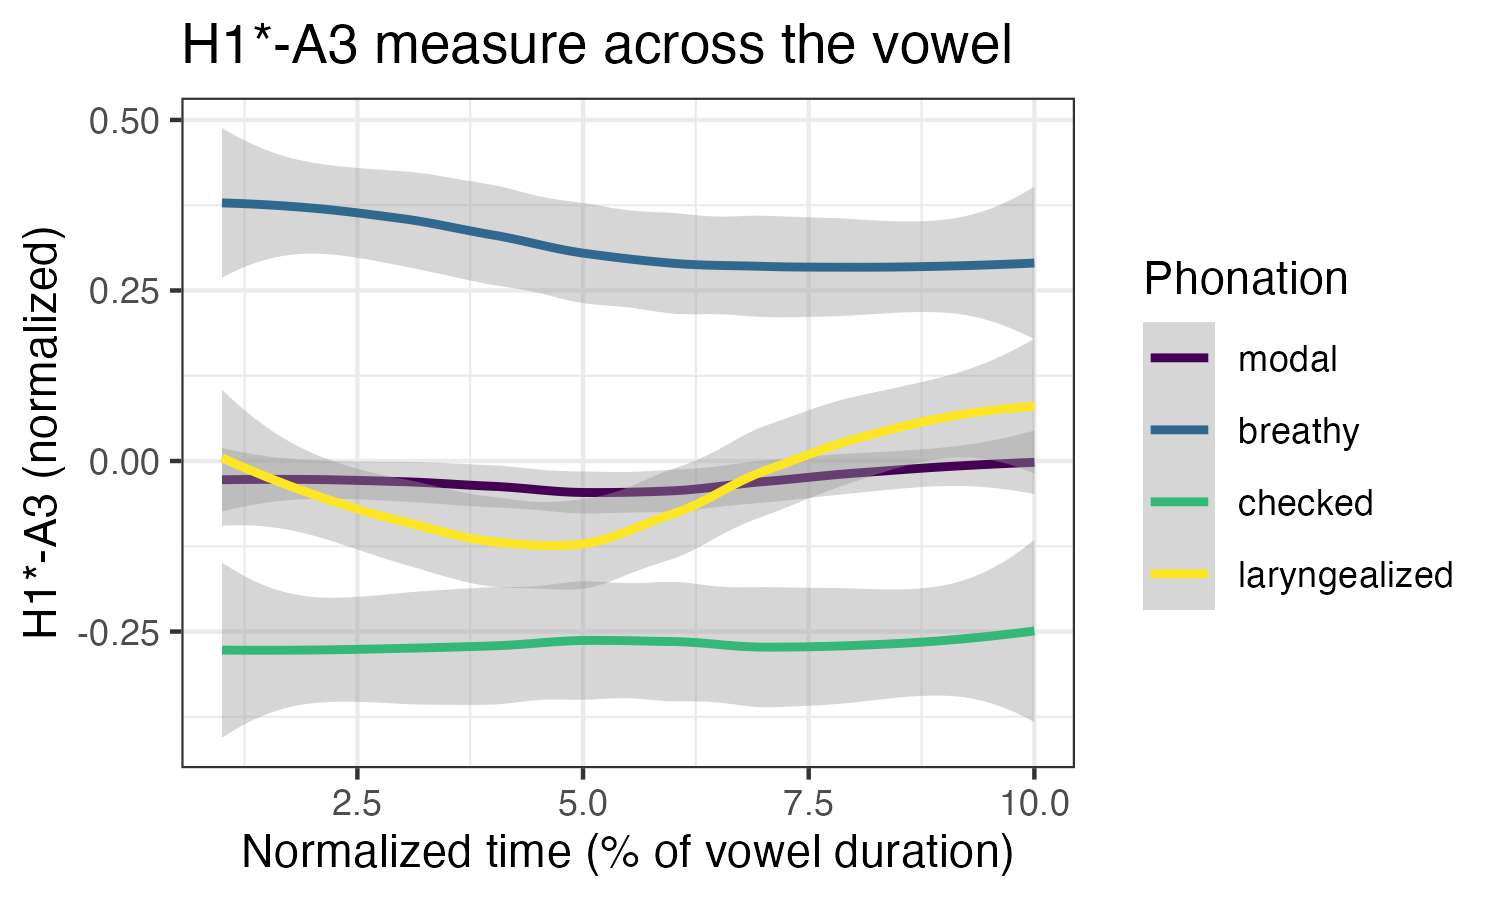
\includegraphics[width=\textwidth]{Images/h1a3_clean_line.png}
  \caption{Smooths for H1*-A3 by phonation contrast}
  \end{minipage}\par
  \vskip\floatsep% normal separation between figures
  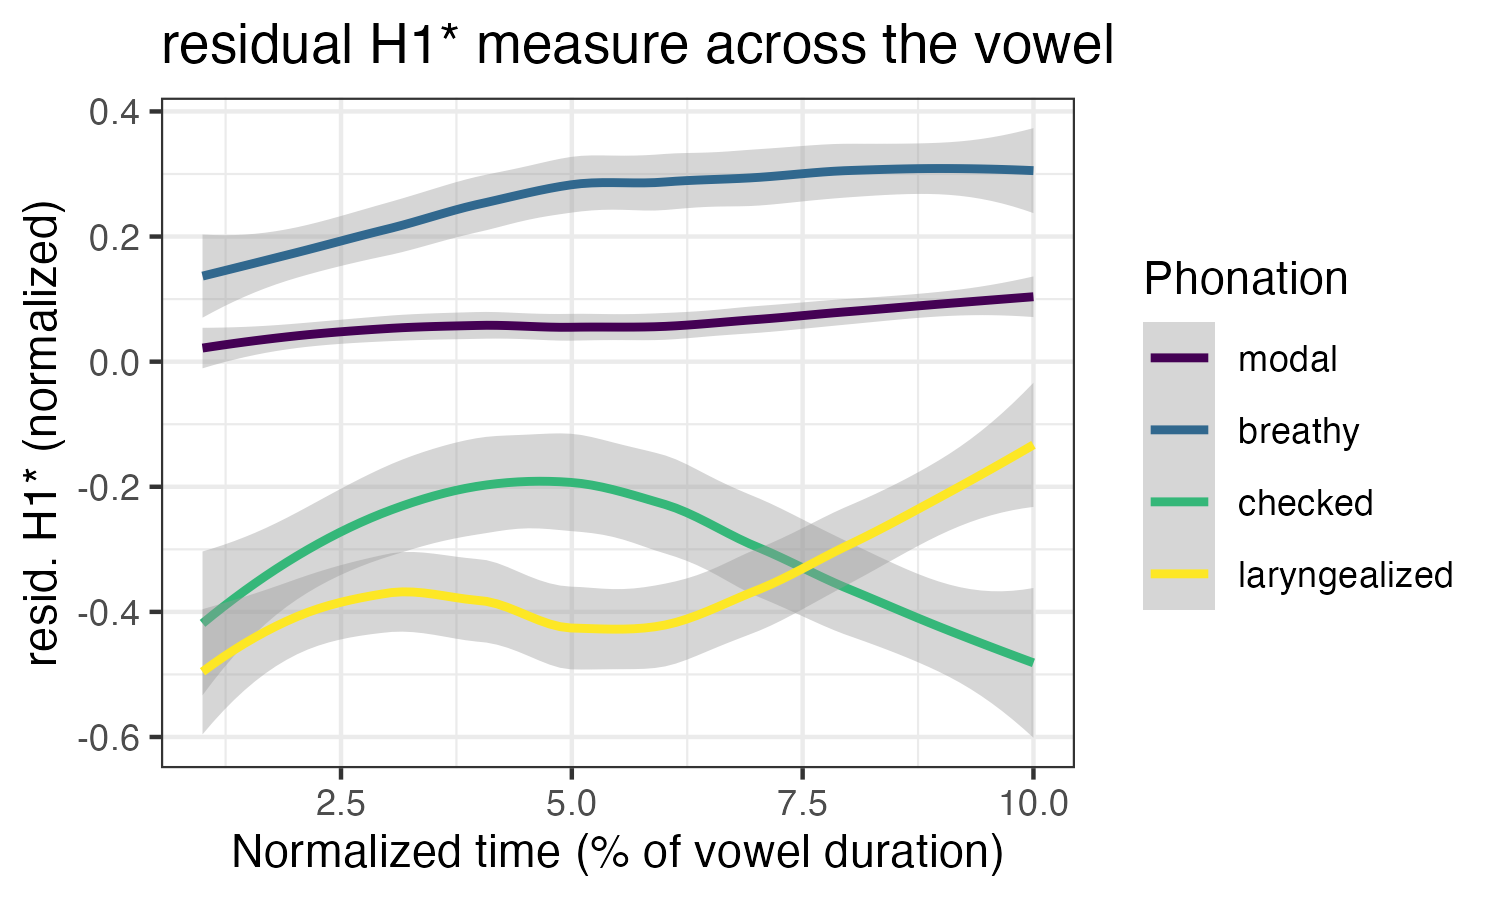
\includegraphics[width=0.45\textwidth]{Images/h1_clean_line.png}
  \caption{Smooths for residual H1* by phonation contrast}
\end{figure}
%\singlespacing
%\nocite{*}
{\printbibliography[heading=bibintoc]}



\end{document}